\documentclass{article}
\usepackage{graphicx} % Required for inserting images
\usepackage{float} % Required for using [H] placement option
\usepackage{algorithm}
\usepackage{algpseudocode}
\usepackage{amsmath}
\usepackage{amsfonts}
\usepackage{amssymb}
\usepackage{authblk}
\usepackage{verbatim}
\usepackage{float}
\usepackage{subcaption}


\title{Gradient Methods for Multi-class Logistic Regression}
\author{Alessandro Pala - 2107800 \and 
Tanner Aaron Graves - 2073559 \and 
Alisa Snezskaia - 2107497 \and
Anna Glado - }

%\affil{Optimization for DataScience, UniPD}
\date{May 2024}

\begin{document}

\maketitle

\section{Introduction}
In this report, we analyze the relative performance of various gradient methods at optimizing a multi-class logistic regression model. Specifically, we are interested in comparing full gradient descent with block coordinate-based methods (BCGD) which optimize one coordinate, or column in parameter matrix $X$, at a time. 

Multi-class logistic classification is an extension of traditional logistic regression. The task goes from predicting a Bernoulli random variable to predicting one label to classify each example from a set of $k$ mutually exclusive labels. We encode the target $b_i \in \mathbb{R}^k$ where $k$ is the number of output classes to be a one-hot array, corresponding to the correct classification of example $a_i \in \mathbb{R}^d$. It assigns these labels by learning the conditional probability distribution that the correct label is $b_i$ given example $a_i$ and learned parameter matrix $X \in \mathbb{R}^{d \times k}$ where $d$ is the number of features in each example. The output distribution is computed with the softmax function in this context: 
$$P(b_i|a_i, X) = \frac{\exp(x_{b_i}^T a_i)}{\sum_{c=1}^k\exp(x_c^T a_i)}$$

Multi-class logistic regression is a simple yet effective method with ubiquitous use. Its training does, however, require learning the parameter matrix $X$, which can be done using various methods like maximum likelihood or gradient descent-based methods. This corresponds to solving the following optimization problem:
$$\min_{x \in \mathbb{R}^{d \times k}} \sum\limits_{i=1}^{m}[-x^T_{b_i}a_i + \log(\sum\limits_{c=1}^k\exp(x_c^T a_i))]$$
which is the cross-entropy of the predicted class distribution and the target label $b_i$. Of importance to the application of gradient methods is this problem's convexity. This is nice for many reasons, but most importantly we can guarantee that a local minimum found by GD methods will be the global minimum.  
In this report we implement these different methods and apply them to various datasets: A synthetic dataset, to test convergence in high-dimensional scenarios, 

\section{Algorithms}
Here we provide an overview of the methods studied. We implemented the various methods in Python using either PyTorch or NumPy. The three implementations are a full Gradient Descent and two Block-Coordinate Gradient Descent methods, one with the Gauss-Southwell rule and one with the randomized rule.  

\subsection{Gradient Descent}
\begin{algorithm}
\caption{Full Gradient Descent}\label{alg:cap}
\begin{algorithmic}
\State Initialize $X_1 \in \mathbb{R}^{d \times k}$
\For{$k = 1, \ldots $}
    \If{$X \in X^*$} \textbf{STOP} (Optimality conditions)
    \State Set $X_{k+1} = x_k - \alpha_k \nabla$
    \EndIf
\EndFor
\end{algorithmic}
\end{algorithm}

\subsection{Block Coordinate Gradient Descent}
BCGD methods are specialized in optimizing high-dimensional problems where calculation of the gradient can be split up into blocks which are easier to compute. These methods exploit the convex nature of the problem to optimize one coordinate at a time and approach the global optimum.

\begin{algorithm}
\caption{BCGD}\label{alg:cap}
\begin{algorithmic}
\State Initialize $X_1 \in \mathbb{R}^{d \times k}$
\For{$k = 1, \ldots $}
    \If{$X \in X^*$} \textbf{STOP} (Optimality conditions)
    \State Select $i_k \in $ block according to some \textbf{RULE}
    \State Set $x_{k+1} = x_k - \alpha_k [\nabla_x f(x_k)]_{i_k}$
    \EndIf
\EndFor
\end{algorithmic}
\end{algorithm}

Above $\alpha_k \geq 0$ is a step size for the $k$th iteration. We later analyze the effect of different methods for calculating this. The choice of \textbf{RULE} will distinguish the Gauss-Southwell and Randomized variants of BCGD. The Gauss-Southwell (GS) rule is a greedy selection method that focuses on the block with the largest gradient component at each iteration. This method involves computing the gradient of the objective function for all blocks and selecting the one with the maximum gradient norm. By updating the block that is expected to provide the greatest improvement in the objective function, the GS rule can lead to faster convergence, especially in problems where gradients vary significantly across blocks. However, the computational cost is higher due to the need to evaluate the full gradient at each step, making this approach more complex and potentially less efficient for high-dimensional problems.

For the GS rule we compute 
$$i_k = {\arg\max}_j ||\nabla_j f(x_k)||$$
Taking $i_k$ uniform random samples to be the block index gives the randomized rule. This method simplifies the implementation and reduces computational cost, as it only requires computing the gradient of the randomly selected block rather than the full gradient.

\section{Step Sizes}
The more theoretical formulations for block coordinate descent methods use line searching to find an optimal point in the direction of the current gradient block. This does well to minimize the number of iterations for convergence by exploiting the convexity of the logistic classification problem. Should the cost cease to decrease over this line search, then a minima has been found on the line, and thus a block has been minimized. Here we visualize the loss over the line search along a gradient block selected at an iteration of BCGD with GS rule with varying step sizes on the synthetic dataset (Figure 1).  
\begin{figure}
    \centering
    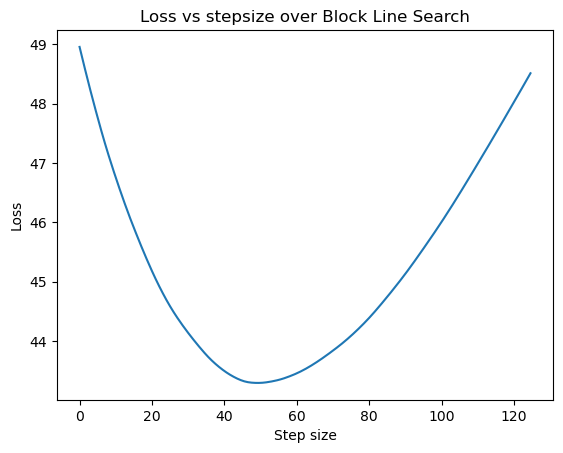
\includegraphics[width=0.5\linewidth]{linesearch.png}
    \caption{Linesearch over one block}
    \label{fig:linesearch}
\end{figure}
In practice, computing he loss at many different points along this line to find the optimal step is a very expensive operation for large datasets. We found that implementing this method proved far too costly
\subsection{Fixed Step Size and the Lipschitz Constant}
Using the inverse of the Lipschitz constant is commonly used in gradient based methods as it guarantees stability. This exploits an assumption we may make about our convex problem to define the a Lipschitz constant $L$, which may be used to ensure that iterations do not overstep minima leading to divergence. It is defined for $x,y$ in the feasible parameter space:
$$L = \max_{x,y} \frac{||\nabla y - \nabla x||_2}{||x - y||_2}$$
and we take stepsize $\alpha=\frac{1}{L}$.
We initially took an empirical approach to approximating $L$ by noting that our initial parameter matrix $X$ had entries iid standard normal, so we sampled many feasible values for $x$ and $y$ and calculated the maximum $L$. This approach, we found, yields fairly reasonable estimates for step size, however, reported consistently larger step sizes that what we found to be optimal. We attribute this to the distribution of parameters changing as a function of iteration. To examine this effect we examine how the optimal step sizes using line searching change with respect to the iteration (figure 2) and magnitude of the gradient block (figure 3). In this scenario, empirical estimation of $L$ gave a step size of $144$, which may have been suitable for initial parameter distributions but not for later values as the plots show.
\begin{figure}[H]
    \centering
    \begin{subfigure}[b]{0.45\linewidth}  % Slightly reduce the width
        \centering
        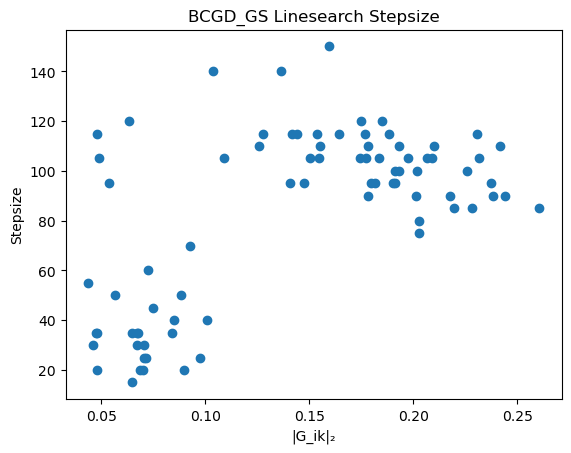
\includegraphics[width=\linewidth]{stepsize_vs_grad_block_norm.png}
        \caption{Comparison of optimal step size versus gradient block norm}
        \label{fig:stepsize_block}
    \end{subfigure}
    \hfill
    \begin{subfigure}[b]{0.45\linewidth}  % Slightly reduce the width
        \centering
        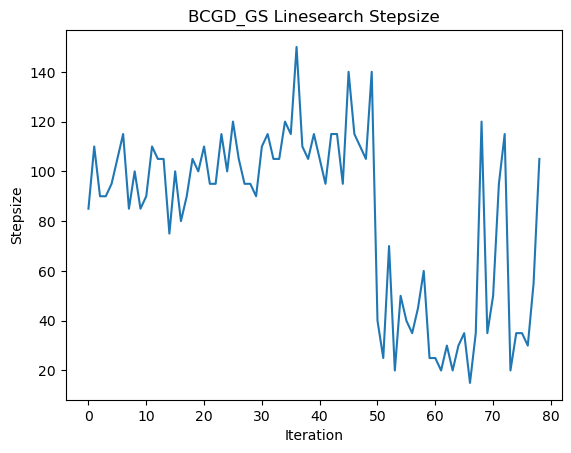
\includegraphics[width=\linewidth]{iter_vs_stepsize.png}
        \caption{Enter Caption}
        \label{fig:enter-label}
    \end{subfigure}
    \caption{Side-by-side comparison of figures}
    \label{fig:side_by_side}
\end{figure}
We moved away from this empirical estimation of $L$ to a more common one in the context of gradient methods: using the maximum eigen-value of the Forbenius-norm of the data matrix $A$.
$$L\approx\max\{|\lambda_i|\} \text{ Where } \lambda_i is an eigen-value of ||A||_F = A^TA$$

\subsection{Block Step Size}
\subsection{Exact Step Size}

\section{Synthetic Dataset}
To initially validate the convergence of our algorithms we generate a high-dimensional dataset for the multi-class classification problem. This consists of our data matrix $A \in \mathbb{R}^{1000 \times 1000}$ and target classes $b$. The rows of $A$ correspond to individual examples in the dataset and the columns their numeric features. Entries for $A$ were drawn i.i.d. from a $N(0,1)$ distribution. Here $b \in \mathbb{Z}_{50}$ represents the vector of target classes corresponding to their respective rows in $A$. We define our starting parameter matrix $X \in \mathbb{R}^{1000 \times 50}$. We can then define an error matrix with standard normal entries to inject noise into our calculation of the target classes
$$b = AX + E$$
and further process $b$ to be the argmax of each row. This dataset has the feature of having an expensive gradient calculation due to the high number of features and output classes. This creates the potential for BCGD methods to be advantaged as ones like the randomized rule may compute a smaller block of the gradient, though this also depends on the generation seed for the distribution.

\subsection{Base Performance}
All the presented results were run at a $6 \times 10^{-6}$ learning rate.\footnote{Testing was done with many learning rate values with all trends remaining almost identical; the chosen value is simply the one that produces the plots that best represent them.}
As for the synthetic dataset, we find that at fixed step size the full gradient outperforms both block-coordinate methods, with the Randomized BCGD performing the worst. In absolute terms, however, all three methods converge to a high accuracy with an efficient CPU time.

\begin{figure}[H]
    \centering
    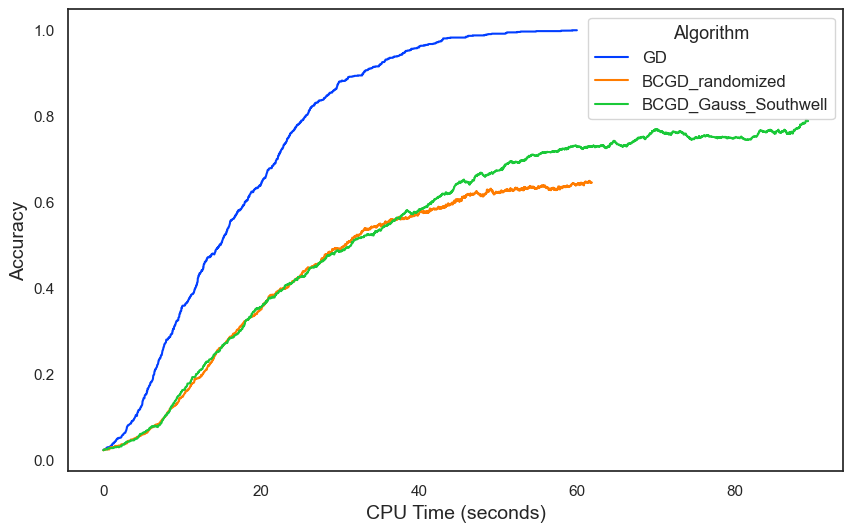
\includegraphics[width=\linewidth]{"C:/Users/alepa/Downloads/Plots/Synthetic_Fixed.png"}
    \caption{Synthetic Dataset - Fixed Step Size}
    \label{fig:synthetic_fixed}
\end{figure}

\subsection{Step Size Analysis}
We also find that the performances of the algorithms remain the same for the other implemented step sizes, with minimal differences solely related to the seed of the distribution and the learning rate. -- Why? --

\begin{figure}[H]
    \centering
    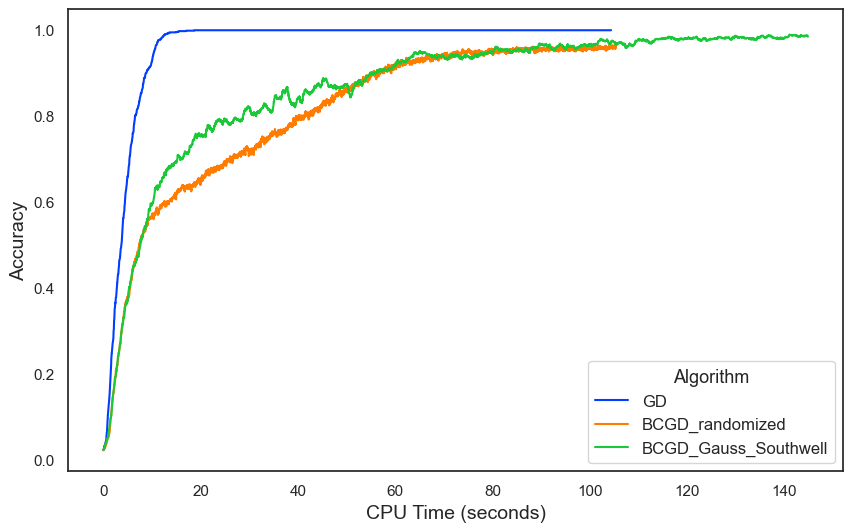
\includegraphics[width=\linewidth]{"C:/Users/alepa/Downloads/Plots/Synthetic_Block.png"}
    \caption{Synthetic Dataset - Block Step Size}
    \label{fig:synthetic_block}
\end{figure}

\begin{figure}[H]
    \centering
    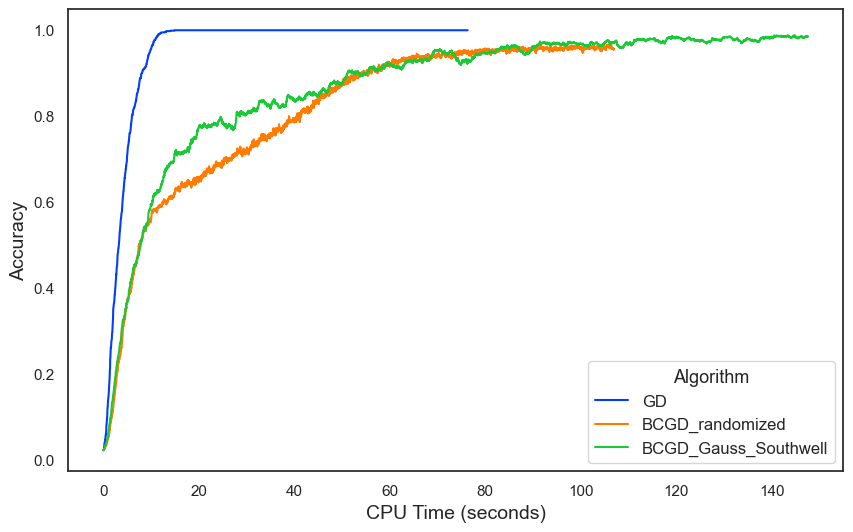
\includegraphics[width=\linewidth]{"C:/Users/alepa/Downloads/Plots/Synthetic_Exact.png"}
    \caption{Synthetic Dataset - Exact Step Size}
    \label{fig:synthetic_exact}
\end{figure}

All step sizes increase indefinitely during descent at roughly the same rate, and all resemble step functions. -- Is this expected? What does it mean? --
\begin{figure}[H]
    \centering
    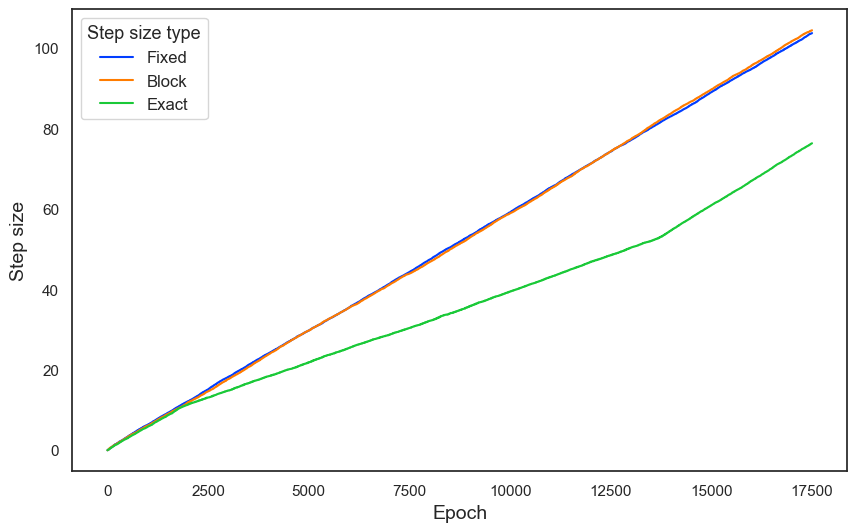
\includegraphics[width=\linewidth]{"C:/Users/alepa/Downloads/Plots/Synthetic_Step_Sizes.png"}
    \caption{Synthetic Dataset - Various Step Sizes}
    \label{fig:synthetic_step_sizes}
\end{figure}


\section{MNIST Dataset}
The MNIST dataset is a large collection of 70,000 labeled handwritten digits in $28\times28$ gray scale. It is widely used for testing models. For the purposes of our use we flatten each example into a vector of length $784$. This dataset was of particular interest to us due to its high dimensionality causing computation of the gradient to be a fairly expensive operation and similarly loss calculation is expensive due in part to the number of examples. This should provide a good opportunity to compare the relative performance of our models. It does, however, have one notable draw back in that the optimization task is not particularly sparse - meaning many coordinates, or features, are important for performance and must be optimized. This is to the detriment of BCGD methods and we aim to examine how much this factor combined with the faster gradient calculation of Randomized BCGD will effect relative performance.
\subsection{Base Performance}
\begin{figure}[H]
    \centering
    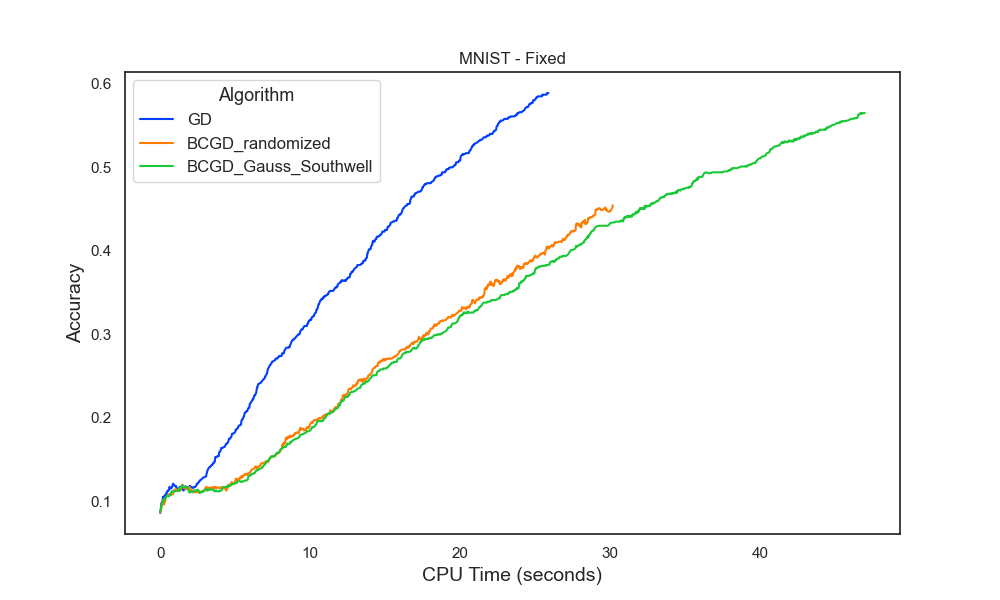
\includegraphics[width=\linewidth]{"C:/Users/alepa/Downloads/Plots/MNIST_Fixed.png"}
    \caption{MNIST Dataset - Fixed Step Size}
    \label{fig:mnist_fixed}
\end{figure}

\subsection{Step Size Analysis}
\begin{figure}[H]
    \centering
    \begin{subfigure}[b]{0.45\linewidth}
        \centering
        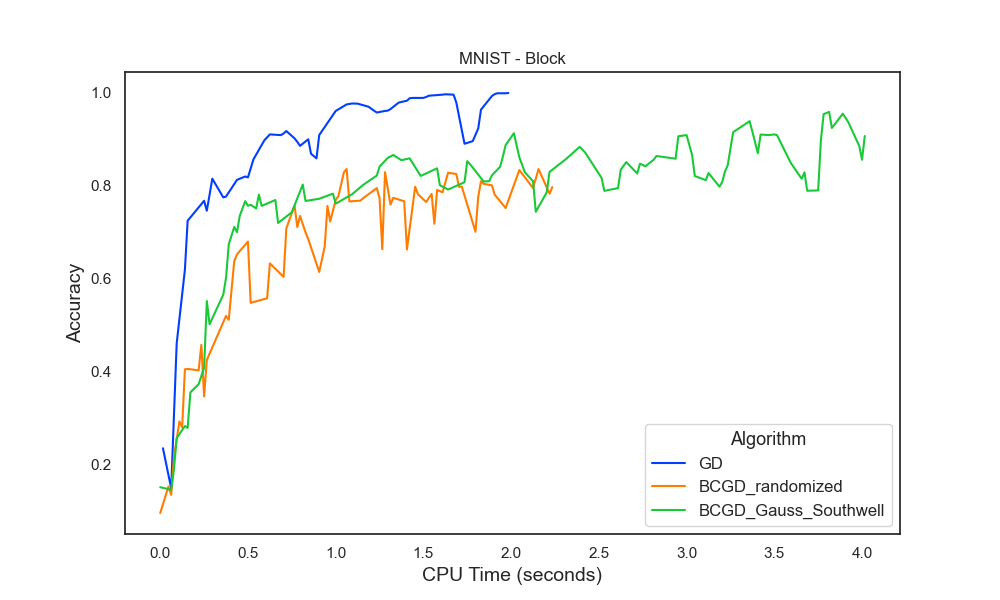
\includegraphics[width=\linewidth]{"C:/Users/alepa/Downloads/Plots/MNIST_Block.png"}
        \caption{MNIST Dataset - Block Step Size}
        \label{fig:mnist_block}
    \end{subfigure}
    \hfill
    \begin{subfigure}[b]{0.45\linewidth}
        \centering
        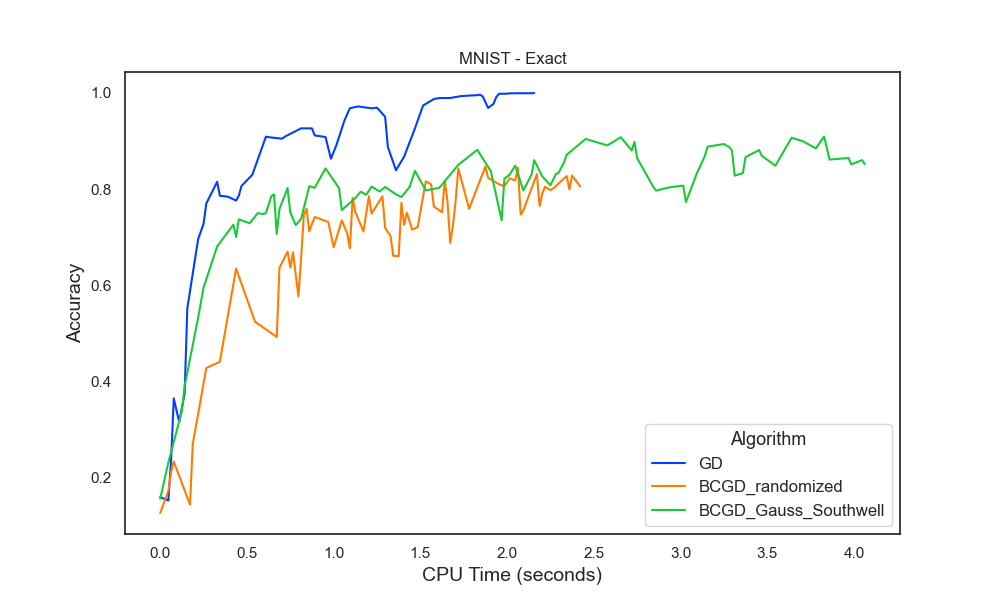
\includegraphics[width=\linewidth]{"C:/Users/alepa/Downloads/Plots/MNIST_Exact.png"}
        \caption{MNIST Dataset - Exact Step Size}
        \label{fig:mnist_exact}
    \end{subfigure}
    \caption{Comparison of MNIST Dataset with Different Step Sizes}
    \label{fig:mnist_comparison}
\end{figure}

\begin{figure}[H]
    \centering
    \includegraphics[width=\linewidth]{"C:/Users/alepa/Downloads/Plots/MNIST_Step_sizes.png"}
    \caption{MNIST Dataset - Various Step Sizes}
    \label{fig:mnist_step_sizes}
\end{figure}

\begin{comment}
\section{Real-world Sparse Dataset}
We selected the MNIST dataset for our first real-world, publicly available dataset. 
\subsection{Base Performance}
\begin{figure}[H]
    \centering
    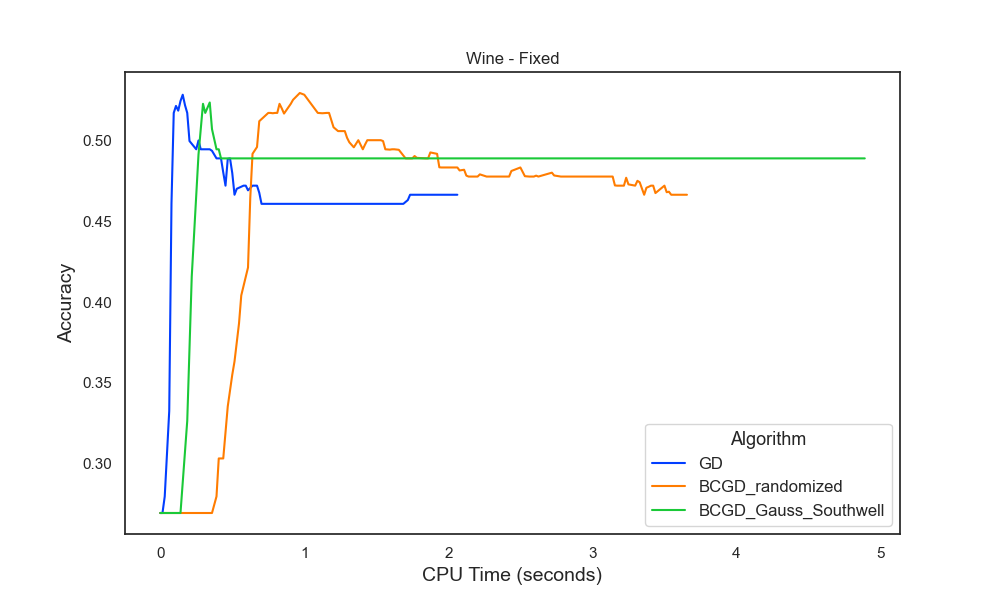
\includegraphics[width=\linewidth]{"C:/Users/alepa/Downloads/Plots/Wine_Fixed.png"}
    \caption{Real-world Sparse Dataset - Fixed Step Size}
    \label{fig:wine_fixed}
\end{figure}

\subsection{Step Size Analysis}
\begin{figure}[H]
    \centering
    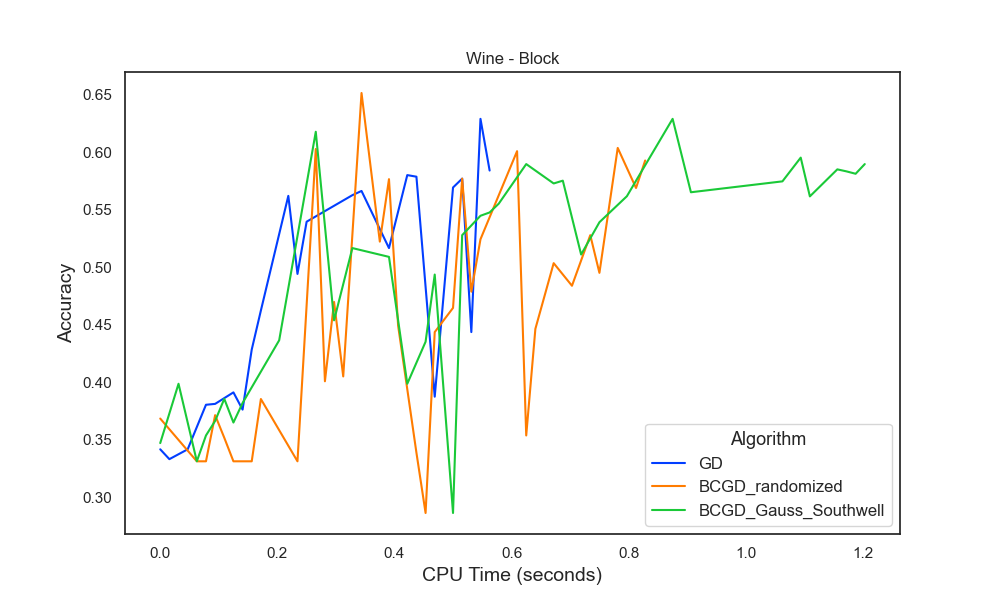
\includegraphics[width=\linewidth]{"C:/Users/alepa/Downloads/Plots/Wine_Block.png"}
    \caption{Real-world Sparse Dataset - Block Step Size}
    \label{fig:wine_block}
\end{figure}

\begin{figure}[H]
    \centering
    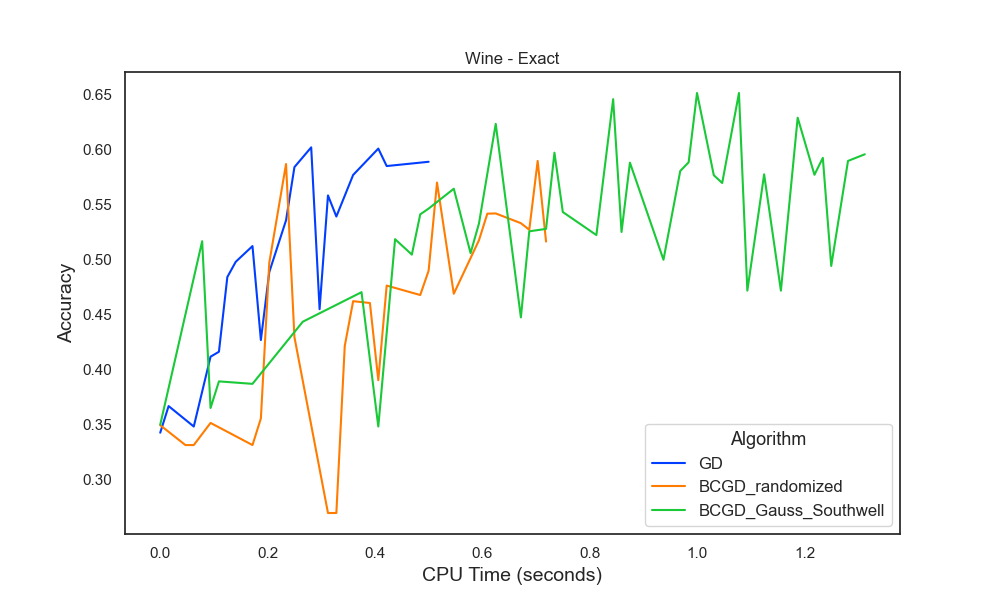
\includegraphics[width=\linewidth]{"C:/Users/alepa/Downloads/Plots/Wine_Exact.png"}
    \caption{Real-world Sparse Dataset - Exact Step Size}
    \label{fig:wine_exact}
\end{figure}

\begin{figure}[H]
    \centering
    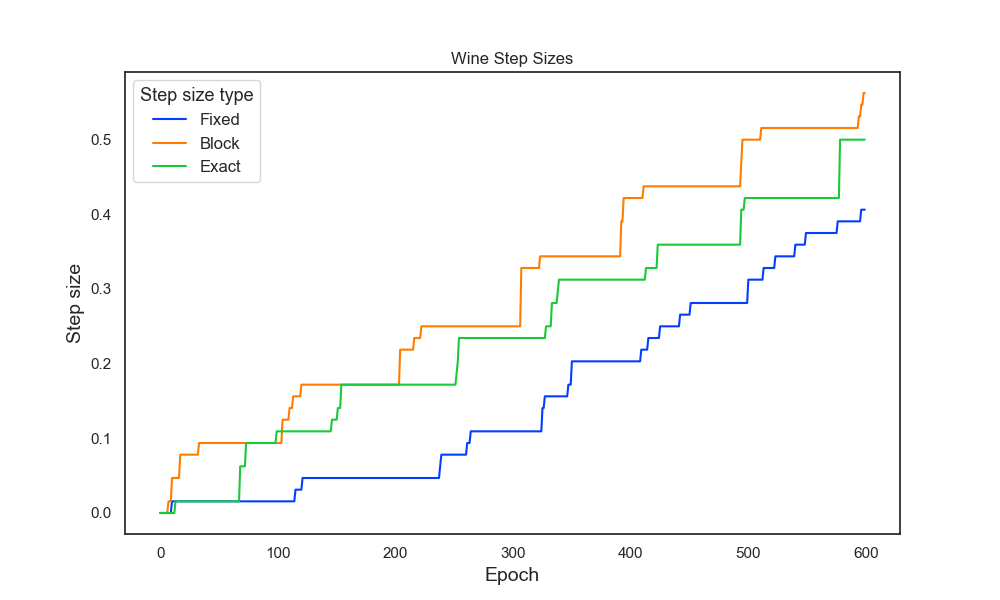
\includegraphics[width=\linewidth]{"C:/Users/alepa/Downloads/Plots/Wine_Step_Sizes.png"}
    \caption{Real-world Sparse Dataset - Various Step Sizes}
    \label{fig:wine_step_sizes}
\end{figure}
\end{comment}

\end{document}
